\section{Kuala Lumpur}

Date: 17/05/2008

\begin{multicols}{2}

On entamme la Malaisie...

Eh oui, nous voici donc en Malaisie, toujours dans le détroit de Malacca séparant l'Indonesie et la Malaisie. Nous avons decide de faire une escale avant Langkawi, notre dernier arrêt avant d'entrer en Thaïlande. Ce sera Port Dickson, proche de Kuala Lumpur (KL pour les intimes). Nous arrivons à Port Dickson et la surprise on nous annonce qu'il y a un gros festival qui va se dérouler pendant les trois jour où nous sommes là, le freedom festival. C'est une sorte d'eurockéennes mais avec que de la musique techno-boum-boum, ils en raffolent ici...

Oui, mais bon, nous c'est pas notre truc... On préfère aller visiter Kuala Lumpur, on se renseigne sur comment y aller : ce sera 1/4h de bus, changement, 1h de bus, puis 1h de train. On nous a dit de descendre à KLCC, c'est là qu'il y a des trucs à voir. En fait il s'agit d'espèces de galeries Lafayettes de luxe : Gucci, Armani, Chanel... Ce qui nous fait croire que KLCC veux dire Kuala Lumpur Chopping Center, si vous avez une autre proposition je suis preneur. Nous pas contrariants, on y va, on sort de la station, on lève les yeux et regardez ce que l'on voit :

\hspace*{-0.65cm}
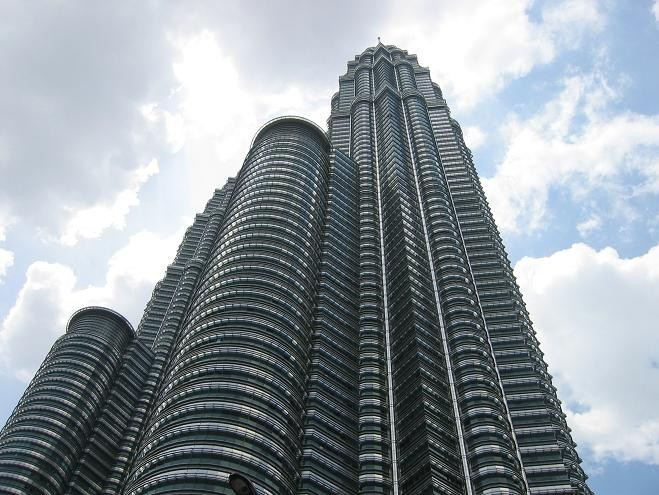
\includegraphics[width=4.8cm]{articles/Kuala-lumpur/1210432312E0e6.jpg}
Tours Petronas

Vous reconnaissez ? c'est les tours jumelles très connues de Kuala Lumpur, elles répondent au petit nom de tours Petronas et sont les tours jumelles encore debout les plus hautes du monde, il paraîtrait qu'il y a une banque au sommet, et c'est ici qu'a été tourné la fin du film Haute Voltige avec Sean Connery.

On continue et qu'est-ce que je vois... un bob AE qui se promène... il paraît qu'il fait le tour du monde (pour ceux qui ne voient pas de quoi je parle, rendez vous à la fin de l'article).

\hspace*{-0.65cm}
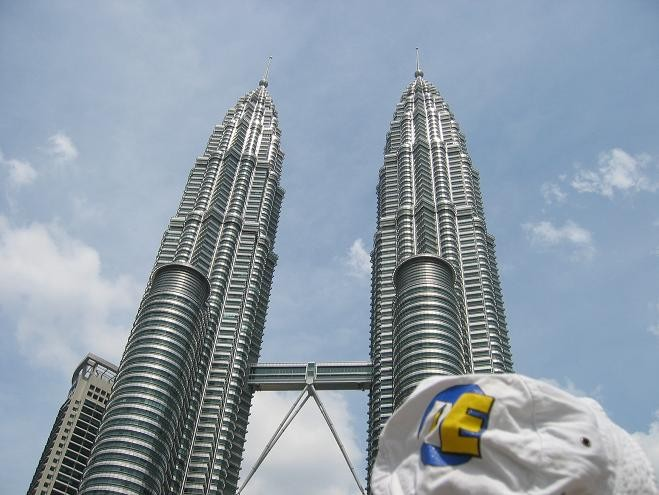
\includegraphics[width=4.8cm]{articles/Kuala-lumpur/1210432316GlgU.jpg}
Tours Petronas again

Allez c'est décidé on marche un peu, on mange un bout, et au detour d'une rue...

\hspace*{-0.65cm}
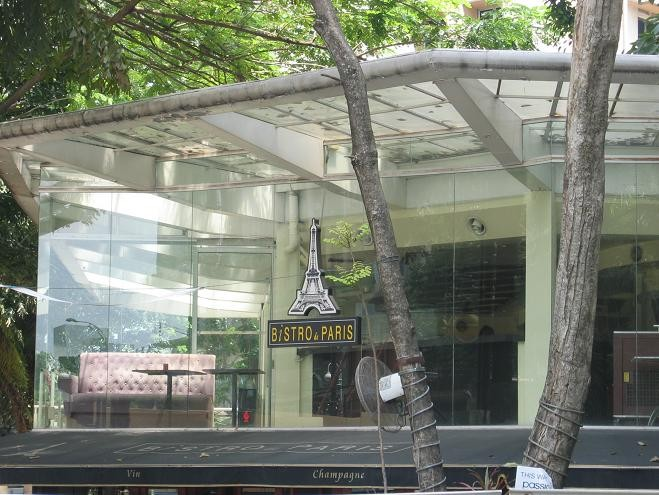
\includegraphics[width=4.8cm]{articles/Kuala-lumpur/1211015560vRGE.jpg}
Un peu de chauvinisme

Y a pas à dire la tour Eiffel et Zidane, restent les deux élément connus partout dans le monde quand on parle de la France.

Bon c'est pas tout ça mais nous on leve encore les yeux au ciel et on voit encore des choses sympa, en particulier cette tour, la 4ème la plus haute du monde avec ses 421 mètres de haut

\hspace*{-0.65cm}
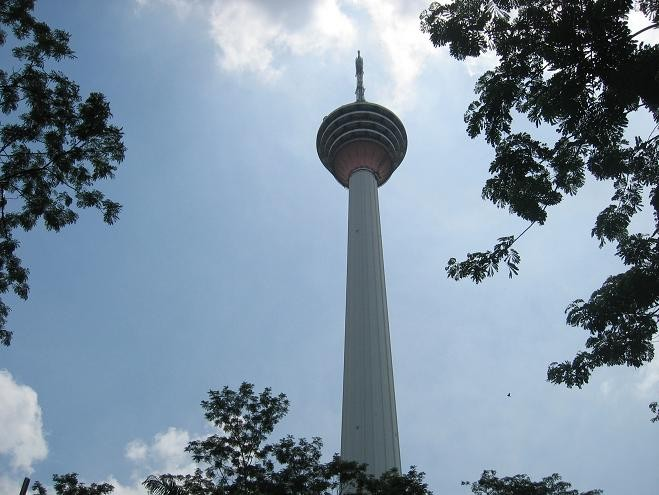
\includegraphics[width=4.8cm]{articles/Kuala-lumpur/1211014906Nl6S.jpg}
Tour qui s'appelle je sais plus comment

Qu'est-ce qu'on doit avoir une belle vue de la haut... allez hop on y va...

\hspace*{-0.65cm}
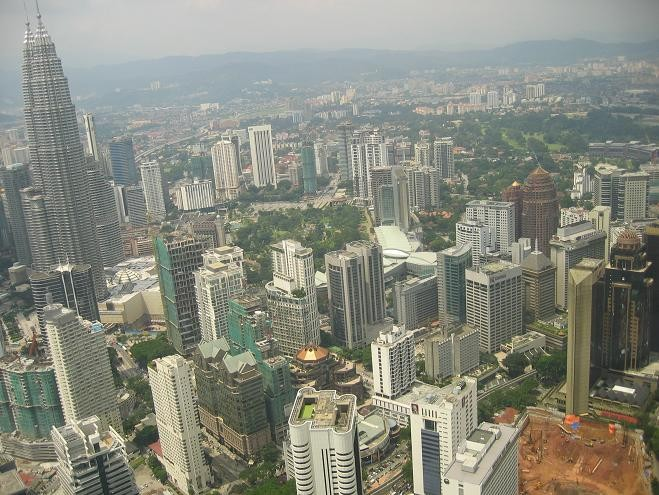
\includegraphics[width=4.8cm]{articles/Kuala-lumpur/1211014913RrBL.jpg}
Vue d'en haut de la tour (qui tourne...)

Moi qui adore voir les choses de loin, et du plus haut possible, j'étais servi. Kuala Lumpur sur 360 degrés.

Retour sur le plancher des singes, en dehors de ses grattes-ciel KL redeviens une ville ressemblant à beaucoup de capitales, si ce n'est que tout est nickel, presque comme à Singapour. Mais allez savoir pourquoi, a KL je me sentais bien, loin de l'impression que j'ai eu à Singapour.

Je vous laisse sur deux photos de la ville en elle même.

\hspace*{-0.65cm}
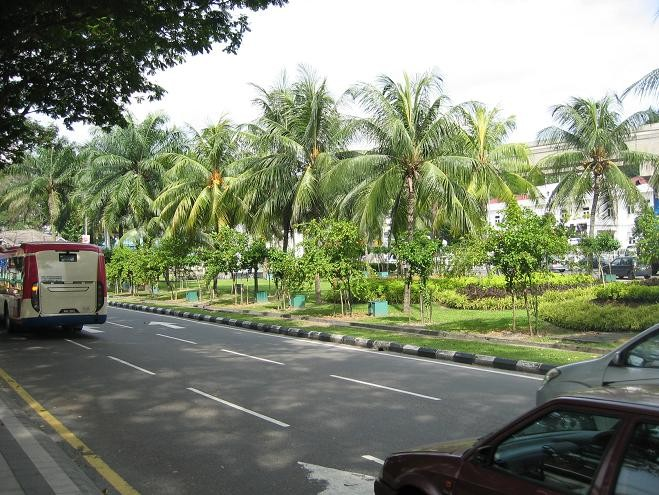
\includegraphics[width=4.8cm]{articles/Kuala-lumpur/1211016874hbIL.jpg}
Ben... la rue quoi

\hspace*{-0.65cm}
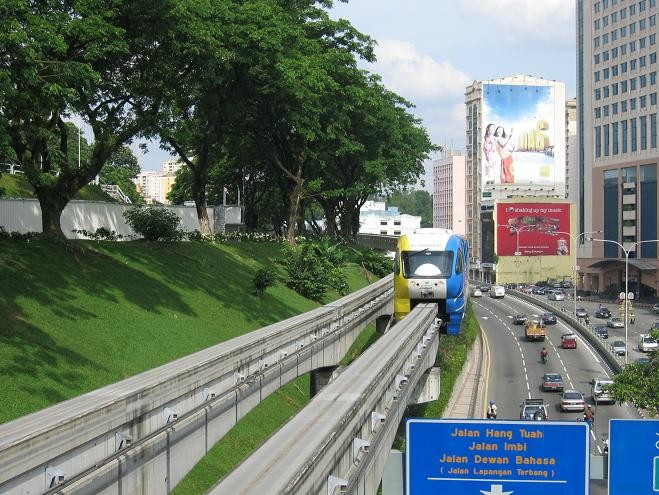
\includegraphics[width=4.8cm]{articles/Kuala-lumpur/1211017229ryCi.jpg}
Monorail aérien

\end{multicols}

 * Le bob autour du monde, kesako ? A l'UTBM il y a eu un message de passé incitant toutes les personnes voyageant autour du monde à emporter un bob AE (Association des Etudiants) et à le prendre en photos devant les grands endroits connus où l'on pourrait aller.
